% Created by tikzDevice version 0.10.1 on 2017-02-07 11:04:04
% !TEX encoding = UTF-8 Unicode
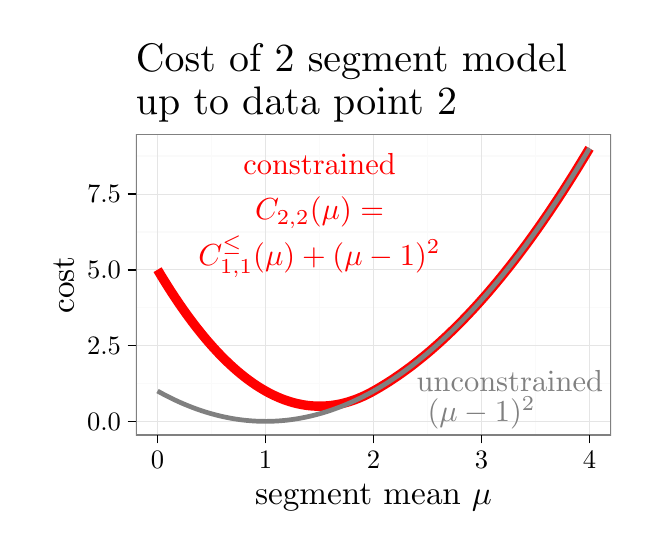
\begin{tikzpicture}[x=1pt,y=1pt]
\definecolor{fillColor}{RGB}{255,255,255}
\path[use as bounding box,fill=fillColor,fill opacity=0.00] (0,0) rectangle (216.81,180.67);
\begin{scope}
\path[clip] (  0.00,  0.00) rectangle (216.81,180.67);
\definecolor{drawColor}{RGB}{255,255,255}
\definecolor{fillColor}{RGB}{255,255,255}

\path[draw=drawColor,line width= 0.6pt,line join=round,line cap=round,fill=fillColor] (  0.00,  0.00) rectangle (216.81,180.68);
\end{scope}
\begin{scope}
\path[clip] ( 39.13, 33.48) rectangle (210.81,142.01);
\definecolor{fillColor}{RGB}{255,255,255}

\path[fill=fillColor] ( 39.13, 33.48) rectangle (210.81,142.01);
\definecolor{drawColor}{gray}{0.98}

\path[draw=drawColor,line width= 0.6pt,line join=round] ( 39.13, 52.11) --
	(210.81, 52.11);

\path[draw=drawColor,line width= 0.6pt,line join=round] ( 39.13, 79.52) --
	(210.81, 79.52);

\path[draw=drawColor,line width= 0.6pt,line join=round] ( 39.13,106.93) --
	(210.81,106.93);

\path[draw=drawColor,line width= 0.6pt,line join=round] ( 39.13,134.33) --
	(210.81,134.33);

\path[draw=drawColor,line width= 0.6pt,line join=round] ( 66.44, 33.48) --
	( 66.44,142.01);

\path[draw=drawColor,line width= 0.6pt,line join=round] (105.46, 33.48) --
	(105.46,142.01);

\path[draw=drawColor,line width= 0.6pt,line join=round] (144.48, 33.48) --
	(144.48,142.01);

\path[draw=drawColor,line width= 0.6pt,line join=round] (183.50, 33.48) --
	(183.50,142.01);
\definecolor{drawColor}{gray}{0.90}

\path[draw=drawColor,line width= 0.2pt,line join=round] ( 39.13, 38.41) --
	(210.81, 38.41);

\path[draw=drawColor,line width= 0.2pt,line join=round] ( 39.13, 65.82) --
	(210.81, 65.82);

\path[draw=drawColor,line width= 0.2pt,line join=round] ( 39.13, 93.22) --
	(210.81, 93.22);

\path[draw=drawColor,line width= 0.2pt,line join=round] ( 39.13,120.63) --
	(210.81,120.63);

\path[draw=drawColor,line width= 0.2pt,line join=round] ( 46.93, 33.48) --
	( 46.93,142.01);

\path[draw=drawColor,line width= 0.2pt,line join=round] ( 85.95, 33.48) --
	( 85.95,142.01);

\path[draw=drawColor,line width= 0.2pt,line join=round] (124.97, 33.48) --
	(124.97,142.01);

\path[draw=drawColor,line width= 0.2pt,line join=round] (163.99, 33.48) --
	(163.99,142.01);

\path[draw=drawColor,line width= 0.2pt,line join=round] (203.01, 33.48) --
	(203.01,142.01);
\definecolor{drawColor}{RGB}{255,0,0}

\path[draw=drawColor,line width= 3.4pt,line join=round] ( 46.93, 93.22) --
	( 47.72, 91.90) --
	( 48.51, 90.60) --
	( 49.30, 89.32) --
	( 50.09, 88.05) --
	( 50.87, 86.80) --
	( 51.66, 85.57) --
	( 52.45, 84.36) --
	( 53.24, 83.16) --
	( 54.03, 81.99) --
	( 54.81, 80.83) --
	( 55.60, 79.69) --
	( 56.39, 78.57) --
	( 57.18, 77.46) --
	( 57.97, 76.37) --
	( 58.76, 75.30) --
	( 59.54, 74.25) --
	( 60.33, 73.22) --
	( 61.12, 72.20) --
	( 61.91, 71.21) --
	( 62.70, 70.23) --
	( 63.49, 69.26) --
	( 64.27, 68.32) --
	( 65.06, 67.39) --
	( 65.85, 66.49) --
	( 66.64, 65.59) --
	( 67.43, 64.72) --
	( 68.21, 63.87) --
	( 69.00, 63.03) --
	( 69.79, 62.21) --
	( 70.58, 61.41) --
	( 71.37, 60.63) --
	( 72.16, 59.86) --
	( 72.94, 59.12) --
	( 73.73, 58.39) --
	( 74.52, 57.68) --
	( 75.31, 56.98) --
	( 76.10, 56.31) --
	( 76.89, 55.65) --
	( 77.67, 55.01) --
	( 78.46, 54.39) --
	( 79.25, 53.78) --
	( 80.04, 53.20) --
	( 80.83, 52.63) --
	( 81.62, 52.08) --
	( 82.40, 51.55) --
	( 83.19, 51.03) --
	( 83.98, 50.54) --
	( 84.77, 50.06) --
	( 85.56, 49.60) --
	( 86.34, 49.15) --
	( 87.13, 48.73) --
	( 87.92, 48.32) --
	( 88.71, 47.93) --
	( 89.50, 47.56) --
	( 90.29, 47.21) --
	( 91.07, 46.87) --
	( 91.86, 46.55) --
	( 92.65, 46.25) --
	( 93.44, 45.97) --
	( 94.23, 45.71) --
	( 95.02, 45.46) --
	( 95.80, 45.23) --
	( 96.59, 45.02) --
	( 97.38, 44.83) --
	( 98.17, 44.66) --
	( 98.96, 44.50) --
	( 99.75, 44.36) --
	(100.53, 44.24) --
	(101.32, 44.14) --
	(102.11, 44.05) --
	(102.90, 43.99) --
	(103.69, 43.94) --
	(104.47, 43.90) --
	(105.26, 43.89) --
	(106.05, 43.90) --
	(106.84, 43.92) --
	(107.63, 43.96) --
	(108.42, 44.02) --
	(109.20, 44.09) --
	(109.99, 44.19) --
	(110.78, 44.30) --
	(111.57, 44.43) --
	(112.36, 44.58) --
	(113.15, 44.74) --
	(113.93, 44.92) --
	(114.72, 45.13) --
	(115.51, 45.35) --
	(116.30, 45.58) --
	(117.09, 45.84) --
	(117.87, 46.11) --
	(118.66, 46.40) --
	(119.45, 46.71) --
	(120.24, 47.04) --
	(121.03, 47.38) --
	(121.82, 47.74) --
	(122.60, 48.12) --
	(123.39, 48.52) --
	(124.18, 48.94) --
	(124.97, 49.37) --
	(124.97, 49.37) --
	(125.76, 49.82) --
	(126.55, 50.28) --
	(127.33, 50.74) --
	(128.12, 51.22) --
	(128.91, 51.70) --
	(129.70, 52.19) --
	(130.49, 52.69) --
	(131.28, 53.20) --
	(132.06, 53.72) --
	(132.85, 54.25) --
	(133.64, 54.79) --
	(134.43, 55.33) --
	(135.22, 55.89) --
	(136.00, 56.45) --
	(136.79, 57.02) --
	(137.58, 57.60) --
	(138.37, 58.19) --
	(139.16, 58.79) --
	(139.95, 59.40) --
	(140.73, 60.02) --
	(141.52, 60.65) --
	(142.31, 61.28) --
	(143.10, 61.93) --
	(143.89, 62.58) --
	(144.68, 63.24) --
	(145.46, 63.91) --
	(146.25, 64.59) --
	(147.04, 65.28) --
	(147.83, 65.98) --
	(148.62, 66.69) --
	(149.41, 67.40) --
	(150.19, 68.13) --
	(150.98, 68.86) --
	(151.77, 69.60) --
	(152.56, 70.36) --
	(153.35, 71.12) --
	(154.13, 71.89) --
	(154.92, 72.66) --
	(155.71, 73.45) --
	(156.50, 74.25) --
	(157.29, 75.05) --
	(158.08, 75.87) --
	(158.86, 76.69) --
	(159.65, 77.52) --
	(160.44, 78.36) --
	(161.23, 79.21) --
	(162.02, 80.07) --
	(162.81, 80.94) --
	(163.59, 81.82) --
	(164.38, 82.70) --
	(165.17, 83.60) --
	(165.96, 84.50) --
	(166.75, 85.41) --
	(167.53, 86.34) --
	(168.32, 87.27) --
	(169.11, 88.21) --
	(169.90, 89.16) --
	(170.69, 90.11) --
	(171.48, 91.08) --
	(172.26, 92.05) --
	(173.05, 93.04) --
	(173.84, 94.03) --
	(174.63, 95.03) --
	(175.42, 96.05) --
	(176.21, 97.07) --
	(176.99, 98.09) --
	(177.78, 99.13) --
	(178.57,100.18) --
	(179.36,101.24) --
	(180.15,102.30) --
	(180.94,103.37) --
	(181.72,104.46) --
	(182.51,105.55) --
	(183.30,106.65) --
	(184.09,107.76) --
	(184.88,108.88) --
	(185.66,110.00) --
	(186.45,111.14) --
	(187.24,112.29) --
	(188.03,113.44) --
	(188.82,114.60) --
	(189.61,115.78) --
	(190.39,116.96) --
	(191.18,118.15) --
	(191.97,119.35) --
	(192.76,120.55) --
	(193.55,121.77) --
	(194.34,123.00) --
	(195.12,124.23) --
	(195.91,125.48) --
	(196.70,126.73) --
	(197.49,127.99) --
	(198.28,129.26) --
	(199.07,130.54) --
	(199.85,131.83) --
	(200.64,133.13) --
	(201.43,134.43) --
	(202.22,135.75) --
	(203.01,137.07);
\definecolor{drawColor}{gray}{0.50}

\path[draw=drawColor,line width= 1.7pt,line join=round] ( 46.93, 49.37) --
	( 48.51, 48.50) --
	( 50.09, 47.67) --
	( 51.66, 46.88) --
	( 53.24, 46.11) --
	( 54.81, 45.39) --
	( 56.39, 44.70) --
	( 57.97, 44.05) --
	( 59.54, 43.43) --
	( 61.12, 42.85) --
	( 62.70, 42.30) --
	( 64.27, 41.79) --
	( 65.85, 41.32) --
	( 67.43, 40.88) --
	( 69.00, 40.48) --
	( 70.58, 40.11) --
	( 72.16, 39.78) --
	( 73.73, 39.48) --
	( 75.31, 39.22) --
	( 76.89, 39.00) --
	( 78.46, 38.81) --
	( 80.04, 38.66) --
	( 81.62, 38.54) --
	( 83.19, 38.46) --
	( 84.77, 38.42) --
	( 86.34, 38.41) --
	( 87.92, 38.44) --
	( 89.50, 38.50) --
	( 91.07, 38.60) --
	( 92.65, 38.73) --
	( 94.23, 38.90) --
	( 95.80, 39.11) --
	( 97.38, 39.35) --
	( 98.96, 39.63) --
	(100.53, 39.94) --
	(102.11, 40.29) --
	(103.69, 40.67) --
	(105.26, 41.10) --
	(106.84, 41.55) --
	(108.42, 42.04) --
	(109.99, 42.57) --
	(111.57, 43.14) --
	(113.15, 43.73) --
	(114.72, 44.37) --
	(116.30, 45.04) --
	(117.87, 45.75) --
	(119.45, 46.49) --
	(121.03, 47.27) --
	(122.60, 48.08) --
	(124.18, 48.93) --
	(125.76, 49.82) --
	(127.33, 50.74) --
	(128.91, 51.70) --
	(130.49, 52.69) --
	(132.06, 53.72) --
	(133.64, 54.79) --
	(135.22, 55.89) --
	(136.79, 57.02) --
	(138.37, 58.19) --
	(139.95, 59.40) --
	(141.52, 60.65) --
	(143.10, 61.93) --
	(144.68, 63.24) --
	(146.25, 64.59) --
	(147.83, 65.98) --
	(149.41, 67.40) --
	(150.98, 68.86) --
	(152.56, 70.36) --
	(154.13, 71.89) --
	(155.71, 73.45) --
	(157.29, 75.05) --
	(158.86, 76.69) --
	(160.44, 78.36) --
	(162.02, 80.07) --
	(163.59, 81.82) --
	(165.17, 83.60) --
	(166.75, 85.41) --
	(168.32, 87.27) --
	(169.90, 89.16) --
	(171.48, 91.08) --
	(173.05, 93.04) --
	(174.63, 95.03) --
	(176.21, 97.07) --
	(177.78, 99.13) --
	(179.36,101.24) --
	(180.94,103.37) --
	(182.51,105.55) --
	(184.09,107.76) --
	(185.66,110.00) --
	(187.24,112.29) --
	(188.82,114.60) --
	(190.39,116.96) --
	(191.97,119.35) --
	(193.55,121.77) --
	(195.12,124.23) --
	(196.70,126.73) --
	(198.28,129.26) --
	(199.85,131.83) --
	(201.43,134.43) --
	(203.01,137.07);
\definecolor{drawColor}{RGB}{255,0,0}

\node[text=drawColor,anchor=base,inner sep=0pt, outer sep=0pt, scale=  1.10] at (105.46,127.79) {constrained};

\node[text=drawColor,anchor=base,inner sep=0pt, outer sep=0pt, scale=  1.10] at (105.46,111.35) {$C_{2,2}(\mu)=$};
\definecolor{drawColor}{gray}{0.50}

\node[text=drawColor,anchor=base west,inner sep=0pt, outer sep=0pt, scale=  1.10] at (140.58, 49.37) {unconstrained};

\node[text=drawColor,anchor=base west,inner sep=0pt, outer sep=0pt, scale=  1.10] at (144.48, 38.41) {$(\mu-1)^2$};
\definecolor{drawColor}{RGB}{255,0,0}

\node[text=drawColor,anchor=base,inner sep=0pt, outer sep=0pt, scale=  1.10] at (105.46, 94.90) {$C^\leq_{1,1}(\mu)+(\mu-1)^2$};
\definecolor{drawColor}{gray}{0.50}

\path[draw=drawColor,line width= 0.6pt,line join=round,line cap=round] ( 39.13, 33.48) rectangle (210.81,142.01);
\end{scope}
\begin{scope}
\path[clip] (  0.00,  0.00) rectangle (216.81,180.67);
\definecolor{drawColor}{RGB}{0,0,0}

\node[text=drawColor,anchor=base east,inner sep=0pt, outer sep=0pt, scale=  0.96] at ( 33.73, 35.10) {0.0};

\node[text=drawColor,anchor=base east,inner sep=0pt, outer sep=0pt, scale=  0.96] at ( 33.73, 62.51) {2.5};

\node[text=drawColor,anchor=base east,inner sep=0pt, outer sep=0pt, scale=  0.96] at ( 33.73, 89.92) {5.0};

\node[text=drawColor,anchor=base east,inner sep=0pt, outer sep=0pt, scale=  0.96] at ( 33.73,117.32) {7.5};
\end{scope}
\begin{scope}
\path[clip] (  0.00,  0.00) rectangle (216.81,180.67);
\definecolor{drawColor}{RGB}{0,0,0}

\path[draw=drawColor,line width= 0.6pt,line join=round] ( 36.13, 38.41) --
	( 39.13, 38.41);

\path[draw=drawColor,line width= 0.6pt,line join=round] ( 36.13, 65.82) --
	( 39.13, 65.82);

\path[draw=drawColor,line width= 0.6pt,line join=round] ( 36.13, 93.22) --
	( 39.13, 93.22);

\path[draw=drawColor,line width= 0.6pt,line join=round] ( 36.13,120.63) --
	( 39.13,120.63);
\end{scope}
\begin{scope}
\path[clip] (  0.00,  0.00) rectangle (216.81,180.67);
\definecolor{drawColor}{RGB}{0,0,0}

\path[draw=drawColor,line width= 0.6pt,line join=round] ( 46.93, 30.48) --
	( 46.93, 33.48);

\path[draw=drawColor,line width= 0.6pt,line join=round] ( 85.95, 30.48) --
	( 85.95, 33.48);

\path[draw=drawColor,line width= 0.6pt,line join=round] (124.97, 30.48) --
	(124.97, 33.48);

\path[draw=drawColor,line width= 0.6pt,line join=round] (163.99, 30.48) --
	(163.99, 33.48);

\path[draw=drawColor,line width= 0.6pt,line join=round] (203.01, 30.48) --
	(203.01, 33.48);
\end{scope}
\begin{scope}
\path[clip] (  0.00,  0.00) rectangle (216.81,180.67);
\definecolor{drawColor}{RGB}{0,0,0}

\node[text=drawColor,anchor=base,inner sep=0pt, outer sep=0pt, scale=  0.96] at ( 46.93, 21.46) {0};

\node[text=drawColor,anchor=base,inner sep=0pt, outer sep=0pt, scale=  0.96] at ( 85.95, 21.46) {1};

\node[text=drawColor,anchor=base,inner sep=0pt, outer sep=0pt, scale=  0.96] at (124.97, 21.46) {2};

\node[text=drawColor,anchor=base,inner sep=0pt, outer sep=0pt, scale=  0.96] at (163.99, 21.46) {3};

\node[text=drawColor,anchor=base,inner sep=0pt, outer sep=0pt, scale=  0.96] at (203.01, 21.46) {4};
\end{scope}
\begin{scope}
\path[clip] (  0.00,  0.00) rectangle (216.81,180.67);
\definecolor{drawColor}{RGB}{0,0,0}

\node[text=drawColor,anchor=base,inner sep=0pt, outer sep=0pt, scale=  1.20] at (124.97,  8.40) {segment mean $\mu$};
\end{scope}
\begin{scope}
\path[clip] (  0.00,  0.00) rectangle (216.81,180.67);
\definecolor{drawColor}{RGB}{0,0,0}

\node[text=drawColor,rotate= 90.00,anchor=base,inner sep=0pt, outer sep=0pt, scale=  1.20] at ( 16.66, 87.74) {cost};
\end{scope}
\begin{scope}
\path[clip] (  0.00,  0.00) rectangle (216.81,180.67);
\definecolor{drawColor}{RGB}{0,0,0}

\node[text=drawColor,anchor=base west,inner sep=0pt, outer sep=0pt, scale=  1.44] at ( 39.13,164.76) {Cost of 2 segment model};

\node[text=drawColor,anchor=base west,inner sep=0pt, outer sep=0pt, scale=  1.44] at ( 39.13,149.21) {up to data point 2};
\end{scope}
\end{tikzpicture}
